\documentclass{beamer}
\usepackage[utf8]{inputenc}

\usetheme{Madrid}
\usecolortheme{default}
\usepackage{amsmath,amssymb,amsfonts,amsthm}
\usepackage{txfonts}
\usepackage{tkz-euclide}
\usepackage{listings}
\usepackage{adjustbox}
\usepackage{array}
\usepackage{tabularx}
\usepackage{gvv}
\usepackage{lmodern}
\usepackage{circuitikz}
\usepackage{tikz}
\usepackage{graphicx}

\setbeamertemplate{page number in head/foot}[totalframenumber]

\usepackage{tcolorbox}
\tcbuselibrary{minted,breakable,xparse,skins}



\definecolor{bg}{gray}{0.95}
\DeclareTCBListing{mintedbox}{O{}m!O{}}{%
  breakable=true,
  listing engine=minted,
  listing only,
  minted language=#2,
  minted style=default,
  minted options={%
    linenos,
    gobble=0,
    breaklines=true,
    breakafter=,,
    fontsize=\small,
    numbersep=8pt,
    #1},
  boxsep=0pt,
  left skip=0pt,
  right skip=0pt,
  left=25pt,
  right=0pt,
  top=3pt,
  bottom=3pt,
  arc=5pt,
  leftrule=0pt,
  rightrule=0pt,
  bottomrule=2pt,
  toprule=2pt,
  colback=bg,
  colframe=orange!70,
  enhanced,
  overlay={%
    \begin{tcbclipinterior}
    \fill[orange!20!white] (frame.south west) rectangle ([xshift=20pt]frame.north west);
    \end{tcbclipinterior}},
  #3,
}
\lstset{
    language=C,
    basicstyle=\ttfamily\small,
    keywordstyle=\color{blue},
    stringstyle=\color{orange},
    commentstyle=\color{green!60!black},
    numbers=left,
    numberstyle=\tiny\color{gray},
    breaklines=true,
    showstringspaces=false,
}
%------------------------------------------------------------
%This block of code defines the information to appear in the
%Title page
\title %optional
{2.8.8}
\date{5 September, 2025}
%\subtitle{A short story}

\author % (optional)
{INDHIRESH S - EE25BTECH11027}



\begin{document}


\frame{\titlepage}
\begin{frame}{Question}
If $\vec{a}$ is a unit vector and $(\vec{x} -\vec{a}).(\vec{x}+\vec{a}) = 8$, then find $|\vec{x}|$\\
\end{frame}
\begin{frame}{allowframebreaks}
\frametitle{Equation}

    \centering
    
    \label{tab:parameters}
Given equation:
\begin{align}
     (\vec{x} -\vec{a}).(\vec{x}+\vec{a}) = 8
\end{align}
The given equation can be written as:
\begin{align}
   \myvec{\Vec{x}-\Vec{a}}^T\myvec{\Vec{x}+\Vec{a}}=8
\end{align}
   
\end{frame}


\begin{frame}{Theoretical Solution}
\begin{align}
    ||\Vec{x}||^2-||\Vec{a}||^2=8
\end{align}
Given that $\Vec{a}$ is a unit vector . So,
\begin{align}
    ||\Vec{a}||=1
\end{align}
Substituting the value of $||\Vec{a}||$ in Eq.3.
\begin{align}
    ||\Vec{x}||^2-1=8
\end{align}



\end{frame}
\begin{frame}
\frametitle{Theoretical Solution}
\begin{align}
    ||\Vec{x}||^2=9
\end{align}
\begin{align}
     ||\Vec{x}||=3
\end{align}

\end{frame}

\begin{frame}
\frametitle{Verification}
For verification let us take:
\begin{align}
    \Vec{x}=\myvec{3\\0}\;\;and\;\;\Vec{a}=\myvec{1\\0}
\end{align}
Let's check whether Eq.2 is satisfied:
\begin{align}
\myvec{\Vec{x}-\Vec{a}}^T\myvec{\Vec{x}+\Vec{a}}= \brak{\myvec{3\\0}-\myvec{1\\0}}^T\brak{\myvec{3\\0}+\myvec{1\\0}}
\end{align}
\begin{align}
    \myvec{\Vec{x}-\Vec{a}}^T\myvec{\Vec{x}+\Vec{a}}= \myvec{2\\0}^T\myvec{4\\0}
\end{align}

\begin{align}
    \myvec{\Vec{x}-\Vec{a}}^T\myvec{\Vec{x}+\Vec{a}}= 8
\end{align}

\end{frame}




\begin{frame}[fragile]
    \frametitle{C Code - Midpoint formula }

    \begin{lstlisting}
#include<stdio.h>

void get_x_coords(float ax, float ay, float *x_out, float *y_out) {
    float mag_x = 3.0f;
    *x_out = mag_x * ax;
    *y_out = mag_x * ay;
}



    \end{lstlisting}
\end{frame}


\begin{frame}[fragile]
    \frametitle{Python Code}
    \begin{lstlisting}
import ctypes
import matplotlib.pyplot as plt
import numpy as np

# Load the shared library
lib = ctypes.CDLL('./magnitude.so')

# Specify argument and return types for the C function
lib.get_x_coords.argtypes = [
    ctypes.c_float, # ax
    ctypes.c_float, # ay
    ctypes.POINTER(ctypes.c_float), # x_out
    ctypes.POINTER(ctypes.c_float)  # y_out
]
lib.get_x_coords.restype = None









    \end{lstlisting}
\end{frame}

\begin{frame}[fragile]
    \frametitle{Python Code}
    \begin{lstlisting}
# Define the unit vector a direction
ax, ay = 1.0, 0.0 # (Choose your direction; this is along x-axis)

x_out = ctypes.c_float()
y_out = ctypes.c_float()

# Call the C function
lib.get_x_coords(ax, ay, ctypes.byref(x_out), ctypes.byref(y_out))

# Prepare points for plotting
origin = np.array([0, 0])
a = np.array([ax, ay]) # Unit vector
x = np.array([x_out.value, y_out.value]) # Solution from C

plt.figure(figsize=(6, 6))











    \end{lstlisting}
\end{frame}

\begin{frame}[fragile]
    \frametitle{Python Code}

    \begin{lstlisting}
# Draw vector a
plt.quiver(origin[0], origin[1], a[0], a[1], angles='xy', scale_units='xy', scale=1, color='green', label='a (unit)')
plt.text(a[0], a[1], f'a({a[0]:.1f}, {a[1]:.1f})', fontsize=10, ha='left', va='bottom')

# Draw vector x
plt.quiver(origin[0], origin[1], x[0], x[1], angles='xy', scale_units='xy', scale=1, color='blue', label='x = 3a')
plt.text(x[0], x[1], f'x({x[0]:.1f}, {x[1]:.1f})', fontsize=10, ha='left', va='bottom')

# Draw origin
plt.scatter(origin[0], origin[1], color='black', s=40)
plt.text(origin[0], origin[1], 'O(0,0)', fontsize=10, ha='left', va='top')





    \end{lstlisting}
\end{frame}
\begin{frame}[fragile]
    \frametitle{Python Code}

    \begin{lstlisting}
plt.xlabel("X-axis")
plt.ylabel("Y-axis")
plt.title("Figure")
plt.legend()
plt.grid(True)
plt.xlim(-1, 4)
plt.ylim(-1, 2)
plt.savefig("/media/indhiresh-s/New Volume/Matrix/ee1030-2025/ee25btech11027/MATGEO/2.8.8/figs/figure1.png")
plt.show()



    \end{lstlisting}
\end{frame}



\begin{frame}{Plot}
    \begin{center}
        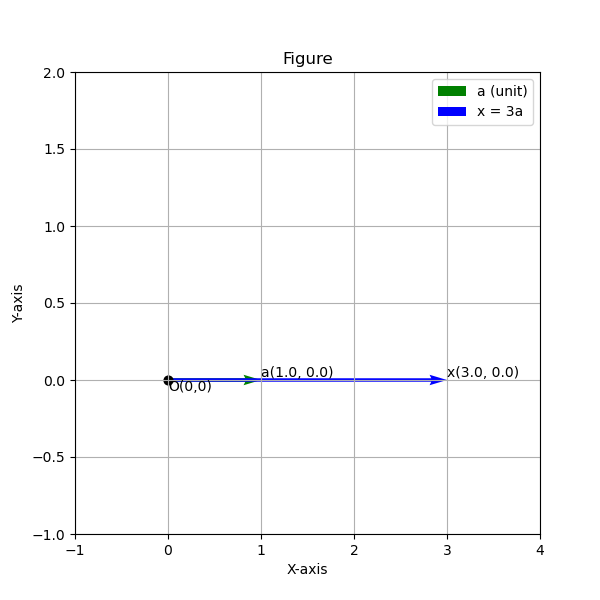
\includegraphics[width=\columnwidth, height=0.8\textheight, keepaspectratio]{figs/figure1.png}
    \end{center}
\end{frame}




\end{document}
